\documentclass[10pt,oneside]{article}

\usepackage[T1]{fontenc}

\usepackage[paper=a4paper,margin=2cm,bottom=2.5cm]{geometry}
\usepackage[sfdefault,light,condensed]{roboto}
\usepackage[export]{adjustbox}
\usepackage[usenames,dvipsnames,table]{xcolor}

\usepackage{amsmath,amssymb,array,fancyhdr,graphicx,enumitem,lastpage,listings,lstautogobble,multicol,tabularx,textcomp,titlesec}
\usepackage{mathtools}

\setlength\parindent{0cm}
\renewcommand\headrule{}
\setlength{\footskip}{1.25cm}


\pagestyle{fancy}

\usepackage{fontawesome,subcaption,tikzsymbols}

% Add some padding to all table cells.
\setlength\extrarowheight{1pt}

%\newcommand{\boxwidth}{\dimexpr\linewidth - 2pt}
\newcommand{\boxwidth}{\linewidth}

\definecolor{BoxHeaderBG}{RGB}{50, 50, 50}
\definecolor{BoxHeaderText}{RGB}{220, 220, 220}

\definecolor{QuestionHeaderBG}{RGB}{200, 200, 200}
\definecolor{QuestionHeaderText}{RGB}{0, 0, 0}

\newcommand{\BoxHeader}[2]{
    \multicolumn{#1}{| >{\bfseries\footnotesize\cellcolor{BoxHeaderBG}\arraybackslash}l |}{
        \textcolor{BoxHeaderText}{#2}
    }
}

\newcounter{QuestionCounter}

\newcommand{\Question}[2]{
    \stepcounter{QuestionCounter}
    \begin{tabularx}{\boxwidth}{|X|}
        \hline
        \cellcolor{QuestionHeaderBG}{\footnotesize\bfseries \textcolor{QuestionHeaderText}{Question \#\theQuestionCounter}} {\em \textcolor{QuestionHeaderText}{#1}} \\\hline
        \ \\[#2]\hline
    \end{tabularx}

    \medskip
}

\newcommand{\FeelQuestion}{
    \stepcounter{QuestionCounter}
    \newcolumntype{F}{>{\centering\arraybackslash}X}
    \begin{tabularx}{\boxwidth}{| F F F |}
        \hline
        \multicolumn{3}{| >{\hsize=\dimexpr3\hsize+4\tabcolsep+2\arrayrulewidth\relax}X |}{
            \cellcolor{QuestionHeaderBG}{\footnotesize\bfseries \textcolor{QuestionHeaderText}{Question \#\theQuestionCounter}} {\em \textcolor{QuestionHeaderText}{Select the option which best reflects how confident you are in applying what you have learend in this lesson.}}}\\\hline
        & & \\[-8pt]
        \Sadey[5][orange] & \Neutrey[5][gray] & \Smiley[5][cyan] \\\hline
    \end{tabularx}

    \medskip
}

\lhead{\tiny\texttt{U\UnitNumber: \UnitTitle\\L\LessonNumber: \LessonTitle}}
\rhead{\tiny\texttt{[DPCS/\CourseLevel/U\UnitNumber/\LessonNumber]\\ }}

\lfoot{
\includegraphics[height=2cm,valign=c]{Files/logo}}
\cfoot{\footnotesize \LessonTitle/DPCS/\CourseLevel/U\UnitNumber/L\LessonNumber/\thepage/\pageref{LastPage}\\Woodstock School/Mussoorie, Uttarakhand, India}
\rfoot{
\includegraphics[height=2cm,valign=c]{Files/ib-world-school-logo-1-colour}}


\def\CourseLevel{SL}

\def\UnitNumber{01}
\def\UnitTitle{The Computer}

\def\LessonNumber{02}
\def\LessonTitle{Storing Data}

\begin{document}
    %Lesson Title
    \begin{center}
        \Large\bfseries \LessonTitle
    \end{center}

    % Objectives List
    \begin{tabularx}{\boxwidth}{|>{\small\raggedleft\bfseries\arraybackslash}p{0.1\textwidth} >{\small\arraybackslash}X |}
        \hline
        \BoxHeader{2}{Objectives} \\\hline
        2.1.9 & Define the terms: bit, byte, binary, denary/decimal, hexadecimal.\\\hline
    \end{tabularx}

    % Opening Exercise
    \section*{Before You Begin}
    The following images show two methods that have been developed for communicating over large distances.

    \begin{figure}[h]
        \centering
        \begin{subfigure}{0.45\boxwidth}
            \centering
            \caption*{Flag Semaphore}
            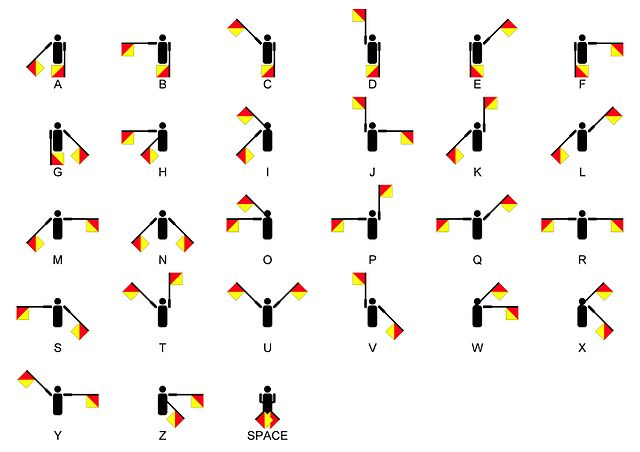
\includegraphics[height=5cm]{Extras/flag_semaphore}
            \caption*{\footnotesize Image courtesy Western University Canada.}
        \end{subfigure}
        \begin{subfigure}{0.45\boxwidth}
            \centering
            \caption*{Morse Code}
            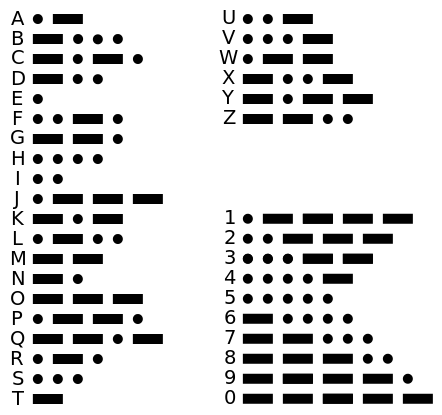
\includegraphics[height=5cm]{Extras/morse_code}
            \caption*{\footnotesize Image courtesy codebug.org.uk.}
        \end{subfigure}
    \end{figure}

    \medskip
    Answer each of the following questions about what you observe in the above communication methods.

    \vfill

    \Question{The telegraph and its associated code were developed in the early 19$^{\text{th}}$ century by Samuel Morse, revolutionizing communications over exceedingly long distances through the use of undersea cables. What makes this code more suitable for communication over electrical circuits than, for instance, the flat semaphore system?}{4cm}

    \Question{One criticism of Morse Code is its lack of consistency in the number of symbols required to represent each character. Why might this cause significant challenges when attempting to adopt its use to computer systems?}{4cm}

    \pagebreak
    
    % Definitions
    \section*{Important Terms}
    \begin{tabularx}{\boxwidth}{| >{\bfseries\arraybackslash}p{0.2\textwidth} | X | }
        \hline
        \BoxHeader{1}{Term} & \BoxHeader{1}{Definition} \\\hline
        Bit & \\[2cm]\hline
        Byte & \\[2cm]\hline
        Binary & \\[2cm]\hline
        Denary / Decimal & \\[2cm]\hline
        Hexadecimal & \\[2cm]\hline
        Number Base & \\[2cm]\hline
        Octal & \\[2cm]\hline
        Word & \\[2cm]\hline
    \end{tabularx}

    \pagebreak

    % Technical Background
    \section*{Technical Background}

    \subsection*{Encoding Information in Bits}
    The following image shows light switches in both an ``ON'' and ``OFF'' position.

    \begin{figure}[h]
        \centering
        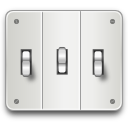
\includegraphics[width=4cm]{Extras/switches}
    \end{figure}

    Consider how these switches, and others like it, can be used to convey information in a way similar to the Morse Code example given in the Opening Exercises.
    \subsubsection*{Notes}

    \vfill

    \Question{Describe a method you could use to encode a negative value using only bits.}{4cm}

    \pagebreak

    \subsection*{Bits \& Bytes}
    Due to the increasingly large amount of data being processed and stored by modern computer systems, prefixes similar to those used by the metric system have been developed for expressing large volumes of data.

    \medskip
    \begin{tabularx}{\boxwidth}{| p{0.1\boxwidth} | X | X |}
        \hline
        \BoxHeader{3}{Units of Information Prefixes} \\\hline
        \BoxHeader{1}{Prefix} & \BoxHeader{1}{Binary Size} & \BoxHeader{1}{Metric Size} \\\hline
        kilo- & & \\[0.5cm]\hline
        mega- & & \\[0.5cm]\hline
        giga- & & \\[0.5cm]\hline
        tera- & & \\[0.5cm]\hline
        peta- & & \\[0.5cm]\hline
        exa- & & \\[0.5cm]\hline
        zetta- & & \\[0.5cm]\hline
        yotta- & & \\[0.5cm]\hline
    \end{tabularx}

    \subsubsection*{Notes}

    \vfill

    \Question{Computer systems store and process information in a series of electronic switches called \emph{transistors}. Over time, these devices have become significantly smaller and fasater, resulting in modern processors containing billions of them. In contrast, a processor from the 1970s would have contained transistors numbering in the thousands. What problems exist due to the sheer quantity of these switches in modern computers?}{4cm}
    
    \pagebreak
    
    \subsection*{Different Number Bases}
    The following table represents the same values in binary, octal, decimal, and hexadecimal.

    \smallskip
    \begin{tabularx}{\boxwidth}{| >{\bfseries\arraybackslash}p{0.125\boxwidth} | X | X | X | X |}
        \hline
        Binary & 1100100 & {\footnotesize 111101000010010000} & {\footnotesize 11110100001001000000} & {\footnotesize 100110001001011010000000} \\\hline
        Octal & 0144 & 0750220 & 03641100 & 046113200 \\\hline
        Decimal & 100 & 250000 & 1000000 & 10000000 \\\hline
        Hexadecimal & 0x64 & 0x3D090 & 0xF4240 & 0x98680 \\\hline
    \end{tabularx}

    \smallskip
    Note the convention of prepending octal values with a `0' and hexadecimal values with `0x'.

    \subsubsection*{Notes}
    \begin{tabularx}{\boxwidth}{| X | X |}
        \hline
        \BoxHeader{1}{Binary $\longrightarrow$ Decimal} & \BoxHeader{1}{Decimal $\longrightarrow$ Binary} \\\hline
        & \\[2cm]\hline
        \BoxHeader{1}{Octal $\longrightarrow$ Decimal} & \BoxHeader{1}{Decimal $\longrightarrow$ Octal} \\\hline
        & \\[2cm]\hline
        \BoxHeader{1}{Hexadecimal $\longrightarrow$ Decimal} & \BoxHeader{1}{Decimal $\longrightarrow$ Hexadecimal} \\\hline
        & \\[2cm]\hline
        \BoxHeader{1}{Binary $\longrightarrow$ Octal} & \BoxHeader{1}{Octal $\longrightarrow$ Binary} \\\hline
        & \\[2cm]\hline
        \BoxHeader{1}{Binary $\longrightarrow$ Hexadecimal} & \BoxHeader{1}{Hexadecimal $\longrightarrow$ Binary} \\\hline
        & \\[2cm]\hline
    \end{tabularx}

    \vfill

    \Question{As discussed, hexadecimal allows for the expression of larger numbers with fewer written digits required. Do you think storage capacities will ever force computer scientists to consider and adopt an even larger base? Why or why not?}{3cm}
    
    \pagebreak
    % Developing Technical Skills
    \section*{Developing Technical Skills}

    \subsubsection*{The ASCII Table}
    The American Standard Code for Information Interchange (ASCII) represents one of the first widely adopted standards for encoding text characters for digital communications. Originally, it used 7-bits to encode 128 characters before being extended into 8-bits, allowing for 256 unique characters. In fact, the first 256 characters of the now common Unicode Standard are exactly the same as in the Extended ASCII table.

    \medskip
    Below is the ASCII table for the capital letters in the standard Latin alphabet. Use it to complete the activity below.

    \begin{center}
        \newcolumntype{C}{>{\centering\arraybackslash}X}
        \begin{tabularx}{0.75\boxwidth}{| C |  C |  C |  C |  C |  C |  C |  C |}
            \BoxHeader{1}{\#} & \BoxHeader{1}{Letter} & \BoxHeader{1}{\#} & \BoxHeader{1}{Letter} & \BoxHeader{1}{\#} & \BoxHeader{1}{Letter} & \BoxHeader{1}{\#} & \BoxHeader{1}{Letter} \\\hline
            65 & A & 72 & H & 79 & O & 86 & V \\\hline
            66 & B & 73 & I & 80 & P & 87 & W \\\hline
            67 & C & 74 & J & 81 & Q & 88 & X \\\hline
            68 & D & 75 & K & 82 & R & 89 & Y \\\hline
            69 & E & 76 & L & 83 & S & 90 & Z \\\hline
            70 & F & 77 & M & 84 & T & \multicolumn{2}{|c|}{\cellcolor{QuestionHeaderBG} }\\\hline
            71 & G & 78 & N & 85 & U & 32 & Space \\\hline
        \end{tabularx}
    \end{center}

    Conver the following binary values to text using the ASCII encoding standard above to read the message. For clarity, each byte is separated by a space.

    \subsubsection*{Binary}
    
    \newcolumntype{T}{>{\ttfamily\centering\arraybackslash}X}
    \begin{tabularx}{\boxwidth}{T T T T T T T T}
        01000011 & 01001111 & 01001101 & 01010000 & 01010101 & 01010100 & 01000101 & 01010010 \\
        00100000 & 01010011 & 01000011 & 01001001 & 01000101 & 01001110 & 01000011 & 01000101 \\
        00100000 & 01001001 & 01010011 & 00100000 & 01000111 & 01010010 & 01000101 & 01000001 \\
        01010100 & & & & & & & 
    \end{tabularx}

    \subsection*{Message}

    \vfill

    \Question{The first 32 characters (0 to 32) in the ASCII standard are reserved for non-printable, command-type characters. For instance, character 2 represents the command ``Start of Test'' and 28 represents ``File Separataor''. Why do you think these characters are necessary for digital communications?}{4cm}

    \pagebreak

    % Reflections
    \section*{Reflections}

    \Question{A \emph{binary coded decimal} value is one which uses binary to express the individual digits in a decimal number. For example, the value $37$ in decimal could be written as $0011$ $0111$ under this scheme. Why do you think this method for encoding numeric values is \emph{not} the standard in computer science?}{4cm}

    \Question{Why is the ASCII encoding standard insufficient for modern communications? Consider the global nature of the Internet and related data transmission networks.}{4cm}

    \Question{Describe at least one new thing you have learned from this lesson. How might you apply this knowledge in the future?}{3.5cm}

    \FeelQuestion

    \Question{What further questions do you still have about this lesson's content?}{3.5cm}
\end{document}